\documentclass[screen, aspectratio=43]{beamer}
\usepackage[T1]{fontenc}
\usepackage[utf8]{inputenc}

\usepackage{xcolor}
\usepackage{listings}

\newcommand{\gfcb}[1]{%
    \fcolorbox{white}{gray!10!}{\quad\strut #1\quad}
    } % gfcb := gray fcolorbox

\usepackage{pgfpages}
\setbeamertemplate{note page}[plain]
\setbeameroption{show notes on second screen=right}

% Use the NTNU-temaet for beamer 
% \usetheme[style=ntnu|simple|vertical|horizontal, 
%     language=bm|nn|en, smalltitle, 
%     city=all|trondheim|alesund|gjovik]{ntnu2017}
\usetheme[style=ntnu,language=en]{ntnu2017}

\usepackage[english]{babel}
\usepackage[style=numeric,backend=biber,natbib=false,sorting=none]{biblatex}
\usepackage{csvsimple}  % for simple table reading and display

\usepackage{booktabs}

\title[Latex Presentations]{How to create Latex Presentations at NTNU}
\subtitle{Using Beamer class}
\author[S. McCallum]{Simon McCallum}
\institute[NTNU]{Department of Computer Sciences, NTNU}
\date{04 October 2017}
%\date{} % To have an empty date

\addbibresource{example.bib} % Add bibliography database

% Set the reference style to numeric.
% See here: http://tex.stackexchange.com/questions/68080/beamer-bibliography-icon
\setbeamertemplate{bibliography item}[text] 

% Set bibliography fonts to a small size.
\renewcommand*{\bibfont}{\footnotesize}


\begin{document}
%-----------------------------------------
\begin{frame}
  \titlepage
\end{frame}

% Alternatively, special title page command to get a different background
% \ntnutitlepage

%-----------------------------------------
\begin{frame}
  \frametitle{Content vs Style}
  \begin{itemize}
      \item {\LaTeX} deals with formatting so you don't have to.
      \item Learn Latex in 30 minutes: \url{https://www.sharelatex.com/learn/Learn_LaTeX_in_30_minutes}
      \item Markup language based on describing content
      \item Uses a container "begin" and "end" model for describing behaviour.
      
  \end{itemize}
    \note{Discuss links to learning on the Sharelatex in 30 minutes\\
    Give examples of markup languages like HTML\\
    Separation of display and content}
\end{frame}

%-----------------------------------------
\begin{frame}
  \frametitle{Thesis Template}
  \begin{itemize}
      \item Github - \url{https://github.com/COPCSE-NTNU}
      \item Masters Thesis, Bachelor Thesis, Beamer (this), and Poster
      \item Provides the layout - DAIM vs Non DAIM
      \item Select your degree short name and language
      \item Includes some macros, \detokenize{\CPP}, \detokenize{\todo} and \detokenize{\com}
      \item 
  \end{itemize}

\end{frame}


%-----------------------------------------
\begin{frame}
  \frametitle{Thesis Template - Data}
  \begin{itemize}
      \item Submission data is given in DAIM webpage
      \item Generating your own - add the content to \gfcb{DaimData.tex}
      \item Generate PDF with \\ \gfcb{\detokenize{\documentclass[MACS,english,DAIM]{ntnuthesis/ntnuthesis}}}
      \item Pretty B5 book cover page
      \item Can include image on the automated system, future feature 
  \end{itemize}
  
    \note{Web based summission\\
   B5 for cost saving on colour printing\\
    }
\end{frame}

%-----------------------------------------
\begin{frame}
  \frametitle{Including files}
  \begin{itemize}
      \item Use file system structure to help you.
      \item Include tex files by path and name
      \item \gfcb{\detokenize{\include{inc/structure}}}
      \item allows logical separation of content
      \item compile only parts of the document
      \item create reusable content
  \end{itemize}
  
    \note{Structure to help organisation\\
   examples\\
    }
\end{frame}

%-----------------------------------------
\begin{frame}
  \frametitle{Including Images}
   \noindent
 \parbox[t]{.75\textwidth}{
  \begin{itemize}
      \item Standard figure includes
      \item Should be in figure environment
  \end{itemize}}
   \hfill
       \raisebox{-.5\height}{
    \includegraphics[width=.2\textwidth]{beamerthementnu2017/figures/kart_student}}
  \begin{itemize}
      \item \gfcb{\detokenize{\includegraphics[width=.2\textwidth]{figures/kart_student}}}
      \item include \gfcb{\detokenize{\caption[short text contents page]{text...}}}
      \item Labels and all Figures must appear with text reference
  \end{itemize}    
    
    \note{\\
    \\
    }

\end{frame}


%-----------------------------------------
\begin{frame}
  \frametitle{Citations}
  \begin{itemize}
      \item Using bibtex important
      \item record abstracts and notes next to reference
      \item Two styles Harvard and Vancouver.  
      \detokenize{\setboolean{HarvardCitations}{false}} 
      \item CS uses Vancouver and so you set Harvard to false
      \item \gfcb{\detokenize{~\cite{Askvall1985}}}
      \item Uses the id from the bibtex file
      \item Can use multiple .bib files
  \end{itemize}
  
    \note{\\
   \\
    }

\end{frame}


%-----------------------------------------
\begin{frame}
  \frametitle{Charts}
  \begin{itemize}
      \item Include as graphics
      \item gnuplot creates nice Latex charts
      \item Use an integrated format psTricks   
      \item Compile graphics inline
      \item Create from a csv file
      \item Scripting for large numbers of charts
      \item Including Latex math in charts
  \end{itemize}
  
    \note{\\
   \\
    }

\end{frame}

%-----------------------------------------
\begin{frame}[fragile]
  \frametitle{Code Listing}
We use the listings package to format code samples nicely

  \begin{figure}[tp] 
  \centering
\lstset{language=Python}
\begin{lstlisting}
import numpy as np
x = 1
a = np.array([[1.0, 2.0], [3.0, 4.0]])
if x == 1:
    # indented four spaces
    print("x is 1.")
    print("Hello World")
    print(a)
\end{lstlisting}
  \caption[Python code example]{The code listing for a Python increment a matrix example}
  \label{fig:PythonCode}
\end{figure}

    \note{\\
   \\
    }

\end{frame}

%-----------------------------------------
\begin{frame}{Math}
The best reason for Latex is the handling of math $4x = 48 $.
\begin{equation} 
\label{H0mean}
    H_0 : \mu_1 = \mu_2
\end{equation}
\end{frame}


%-----------------------------------------
\begin{frame}[fragile]
  \frametitle{Tables}
  \begin{itemize}
      \item Tables are annoying in Latex
      \item We use booktables
      \item \gfcb{\detokenize{\csvautobooktabular{figures/ageiq.csv}}}  
      \item Use tables when text will not do
  \end{itemize}
  
  \begin{table}[tbp]
  \centering
  \csvautobooktabular{figures/ageiq.csv}
  \caption{An example table using simplecsv.}
  \label{tab:examplecsv}
\end{table}
  
    \note{\\
   \\
    }

\end{frame}

%-----------------------------------------
\begin{frame}
  \frametitle{Proof formats}
  \begin{theorem}
    {\LaTeX} makes things easier.
  \end{theorem}

  \begin{proof}
    For details, see Flynn~\cite{latex}.
  \end{proof}
\end{frame}


%-----------------------------------------
\begin{frame}
  \frametitle{References}
  \printbibliography
\end{frame}

\end{document}
